\documentclass[crop,tikz]{standalone}
\begin{document}
    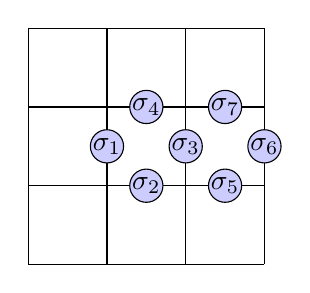
\begin{tikzpicture}[
        baseline={([yshift=-0.5ex]current bounding box.center)},
        site/.style={circle,draw,fill=blue!20,minimum size=#1,
            inner sep=0pt, outer sep=0pt},
        site/.default=12pt
    ]
        \draw (0, 0) -- (0, 1);
        \draw (0, 1) -- (0, 2);
        \draw (0, 2) -- (0, 3);
        \draw (1, 0) -- (1, 1);
        \draw (1, 1) -- node[site] {$\sigma_1$} (1, 2);
        \draw (1, 2) -- (1, 3);
        \draw (2, 0) -- (2, 1);
        \draw (2, 1) -- node[site] {$\sigma_3$} (2, 2);
        \draw (2, 2) -- (2, 3);
        \draw (3, 0) -- (3, 1);
        \draw (3, 1) -- node[site] {$\sigma_6$} (3, 2);
        \draw (3, 2) -- (3, 3);
        \draw (0, 0) -- (1, 0);
        \draw (0, 1) -- (1, 1);
        \draw (0, 2) -- (1, 2);
        \draw (0, 3) -- (1, 3);
        \draw (1, 0) -- (2, 0);
        \draw (1, 1) -- node[site] {$\sigma_2$} (2, 1);
        \draw (1, 2) -- node[site] {$\sigma_4$} (2, 2);
        \draw (1, 3) -- (2, 3);
        \draw (2, 0) -- (3, 0);
        \draw (2, 1) -- node[site] {$\sigma_5$} (3, 1);
        \draw (2, 2) -- node[site] {$\sigma_7$} (3, 2);
        \draw (2, 3) -- (3, 3);
    \end{tikzpicture} \quad = \quad
    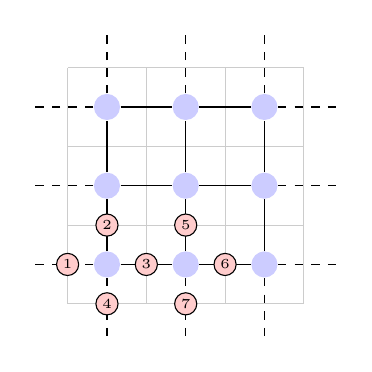
\begin{tikzpicture}[
            baseline={([yshift=-0.5ex]current bounding box.center)},
            leg/.style={
                circle,draw,fill=red!20,minimum size=#1,
                inner sep=0pt, outer sep=0pt,
            },
            leg/.default=8pt,
        ]
        % lattice
        \draw[black!20] (0, 0) -- (0, 1);
        \draw[black!20] (0, 1) -- (0, 2);
        \draw[black!20] (0, 2) -- (0, 3);
        \draw[black!20] (1, 0) -- (1, 1);
        \draw[black!20] (1, 1) -- (1, 2);
        \draw[black!20] (1, 2) -- (1, 3);
        \draw[black!20] (2, 0) -- (2, 1);
        \draw[black!20] (2, 1) -- (2, 2);
        \draw[black!20] (2, 2) -- (2, 3);
        \draw[black!20] (3, 0) -- (3, 1);
        \draw[black!20] (3, 1) -- (3, 2);
        \draw[black!20] (3, 2) -- (3, 3);
        \draw[black!20] (0, 0) -- (1, 0);
        \draw[black!20] (0, 1) -- (1, 1);
        \draw[black!20] (0, 2) -- (1, 2);
        \draw[black!20] (0, 3) -- (1, 3);
        \draw[black!20] (1, 0) -- (2, 0);
        \draw[black!20] (1, 1) -- (2, 1);
        \draw[black!20] (1, 2) -- (2, 2);
        \draw[black!20] (1, 3) -- (2, 3);
        \draw[black!20] (2, 0) -- (3, 0);
        \draw[black!20] (2, 1) -- (3, 1);
        \draw[black!20] (2, 2) -- (3, 2);
        \draw[black!20] (2, 3) -- (3, 3);

        % tensor network
        \draw node[shape=circle,fill=blue!20] (T1) at (0.5, 0.5) {};
        \draw node[shape=circle,fill=blue!20] (T2) at (0.5, 1.5) {};
        \draw node[shape=circle,fill=blue!20] (T3) at (0.5, 2.5) {};

        \draw node[shape=circle,fill=blue!20] (T4) at (1.5, 0.5) {};
        \draw node[shape=circle,fill=blue!20] (T5) at (1.5, 1.5) {};
        \draw node[shape=circle,fill=blue!20] (T6) at (1.5, 2.5) {};

        \draw node[shape=circle,fill=blue!20] (T7) at (2.5, 0.5) {};
        \draw node[shape=circle,fill=blue!20] (T8) at (2.5, 1.5) {};
        \draw node[shape=circle,fill=blue!20] (T9) at (2.5, 2.5) {};
        \draw (T1) -- (T2) -- (T3);
        \draw (T4) -- (T5) -- (T6);
        \draw (T7) -- (T8) -- (T9);

        \draw (T1) -- (T4) -- (T7);
        \draw (T2) -- (T5) -- (T8);
        \draw (T3) -- (T6) -- (T9);

        \draw[dashed] (T1) -- (-0.5, 0.5);
        \draw[dashed] (T2) -- (-0.5, 1.5);
        \draw[dashed] (T3) -- (-0.5, 2.5);

        \draw[dashed] (T1) -- (0.5, -0.5);
        \draw[dashed] (T4) -- (1.5, -0.5);
        \draw[dashed] (T7) -- (2.5, -0.5);

        \draw[dashed] (T7) -- (3.5, 0.5);
        \draw[dashed] (T8) -- (3.5, 1.5);
        \draw[dashed] (T9) -- (3.5, 2.5);

        \draw[dashed] (T3) -- (0.5, 3.5);
        \draw[dashed] (T6) -- (1.5, 3.5);
        \draw[dashed] (T9) -- (2.5, 3.5);

        \draw node[leg] at (0.5, 1) {\tiny 2};
        \draw node[leg] at (1, 0.5) {\tiny 3};
        \draw node[leg] at (0.5, 0) {\tiny 4};
        \draw node[leg] at (0, 0.5) {\tiny 1};

        \draw node[leg] at (1.5, 1) {\tiny 5};
        \draw node[leg] at (2, 0.5) {\tiny 6};
        \draw node[leg] at (1.5, 0) {\tiny 7};
    \end{tikzpicture}
\end{document}
